%!TEX root = cours.tex
\chapter{Tests et conditions}
\introduction{Ceci n'est pas un test !}
\section{Des outils pour comparer}

Ce sont les \textit{opérateurs de comparaison} :\\

{\small
\alternaterowcolors
\begin{tabular}{ccc}
	\rowcolor{lightgray}
	\rowcolor{UGLiOrange}{\boxfont\color{white} Opérateur} & {\boxfont\color{white} Signification} & {\boxfont\color{white} Remarques}                                                                     \\

	\pythoninline{<}                                       & strictement inférieur                 & Ordre usuel sur \pythoninline{int} et \pythoninline{float}, lexicographique sur \pythoninline{str}... \\

	\pythoninline{<=}                                      & inférieur ou égal                     & Idem                                                                                                  \\

	\pythoninline{>}                                       & strictement supérieur                 & Idem                                                                                                  \\

	\pythoninline{>=}                                      & supérieur ou égal                     & Idem                                                                                                  \\

	\pythoninline{==}                                      & égal                                  & \og avoir même valeur\fg\  \textit{Attention :} deux signes =                                         \\

	\pythoninline{!=}                                      & différent                             &                                                                                                       \\

	\pythoninline{is}                                      & identique                             & être le même objet                                                                                    \\

	\pythoninline{is not}                                  & non identique                         &                                                                                                       \\

	\pythoninline{in}                                      & appartient à                          & avec \pythoninline{str}, \pythoninline{list} et \pythoninline{dict}                                   \\

	\pythoninline{not in}                                  & n'appartient pas à                    & avec \pythoninline{str} et \pythoninline{list} et \pythoninline{dict}                                 \\
\end{tabular}
}\normalsize

\begin{pys}
	\begin{minted}{python}
>>> a = 2
>>> a == 2
>>> a == 3
>>> a == 2.0
>>> a is 2.0
>>> a != 100
>>> a > 2
>>> a >= 2
    \end{minted}
\end{pys}

\begin{pys}
	\begin{minted}{python}
>>> a = 'Alice'
>>> b = 'Bob'
>>> a < b
>>> 'e' in a
>>> 'e' in b
>>> liste = [1,10,100]
>>> 2 in liste
    \end{minted}
\end{pys}

Ces opérateurs permettent de réaliser des tests basiques. Pour des tests plus évolués on utilisera des \og mots de liaison \fg{} logiques.

\section{Les connecteurs logiques}

\begin{itemize}
	\item   \pythoninline{and} permet de vérifier que 2 conditions sont \textit{vérifiées simultanément}.
	\item   \pythoninline{or} permet de vérifier qu'\textit{au moins une} des deux conditions est vérifiée.
	\item   \pythoninline{not} est un opérateur de \textit{négation} très utile quand on veut par exemple vérifier qu'une condition est fausse.
\end{itemize}
Voici les tables de vérité des deux premiers connecteurs :

\begin{center}
	\begin{tabular}{|c|c|c|}
		\hline
		\pythoninline{and} & \textit{True}        & \textit{False}       \\
		\hline
		\textit{True}      & \pythoninline{True}  & \pythoninline{False} \\
		\hline
		\textit{False}     & \pythoninline{False} & \pythoninline{False} \\
		\hline
	\end{tabular}\hspace{2em}
	\begin{tabular}{|c|c|c|}
		\hline
		\pythoninline{or} & \textit{True}       & \textit{False}       \\
		\hline
		\textit{True}     & \pythoninline{True} & \pythoninline{True}  \\
		\hline
		\textit{False}    & \pythoninline{True} & \pythoninline{False} \\
		\hline
	\end{tabular}
\end{center}
À ceci on peut ajouter que \pythoninline{not True} vaut \pythoninline{False} et vice-versa.

\begin{pys}
	\begin{minted}{python}
>>> True and False
>>> True or False
>>> not True
    \end{minted}
\end{pys}

\begin{pys}
	\begin{minted}{python}
>>> resultats = 12.8
>>> mention_bien = resultats >= 14 and resultats < 16
>>> print(mention_bien)
    \end{minted}
\end{pys}

\section{if, else et elif}
Voici le schéma de fonctionnement d'un test \pythoninline{if} :
\begin{center}
	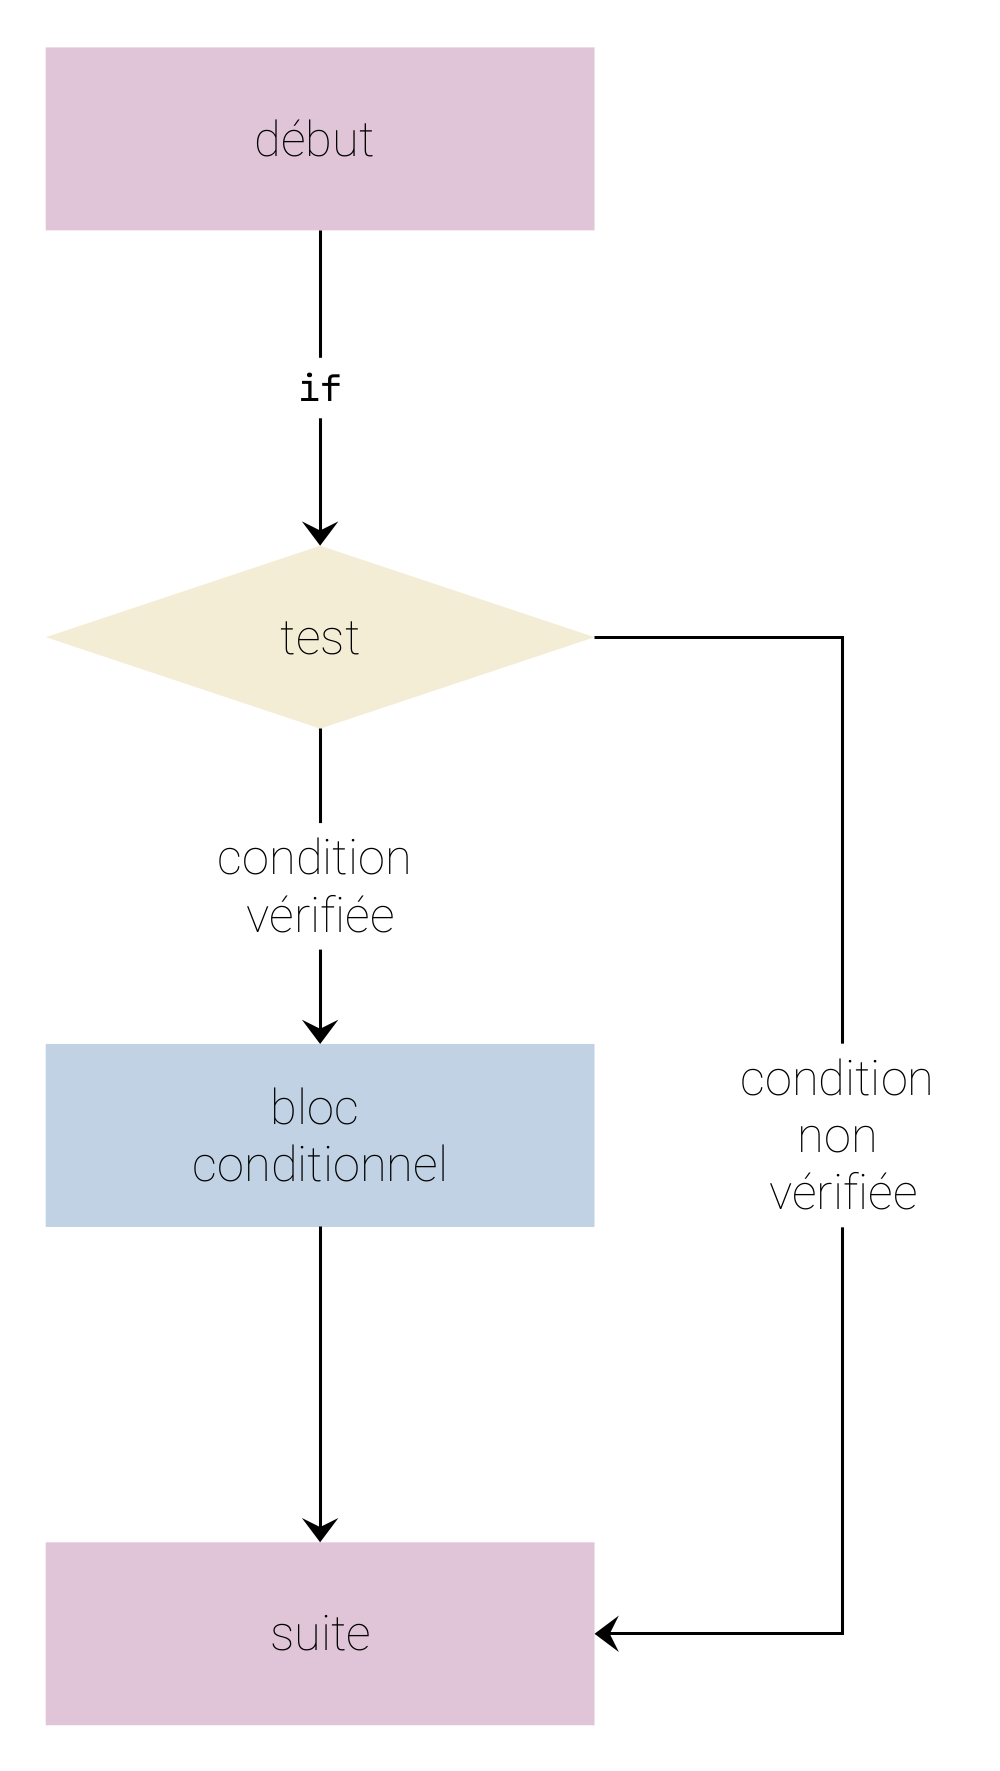
\includegraphics[height=10cm]{img/if}
\end{center}

\textbf{Attention :} Un bloc conditionnel doit être \textit{tabulé} par rapport à la ligne précédente : il n'y a ni \pythoninline{DébutSi}  ni \pythoninline{FinSi}
en \textsc{Python}, ce sont les tabulations qui délimitent les blocs.

\begin{pyc}
	\begin{minted}{python}
phrase='Je vous trouve très joli'
reponse = input('Etes vous une femme ?(O/N) : ')
if reponse == 'O':
    phrase += 'e'
phrase +='.'
print(phrase)
\end{minted}
\end{pyc}

Voici le schéma de fonctionnement d'un test \pythoninline{if...else} :
\begin{center}
	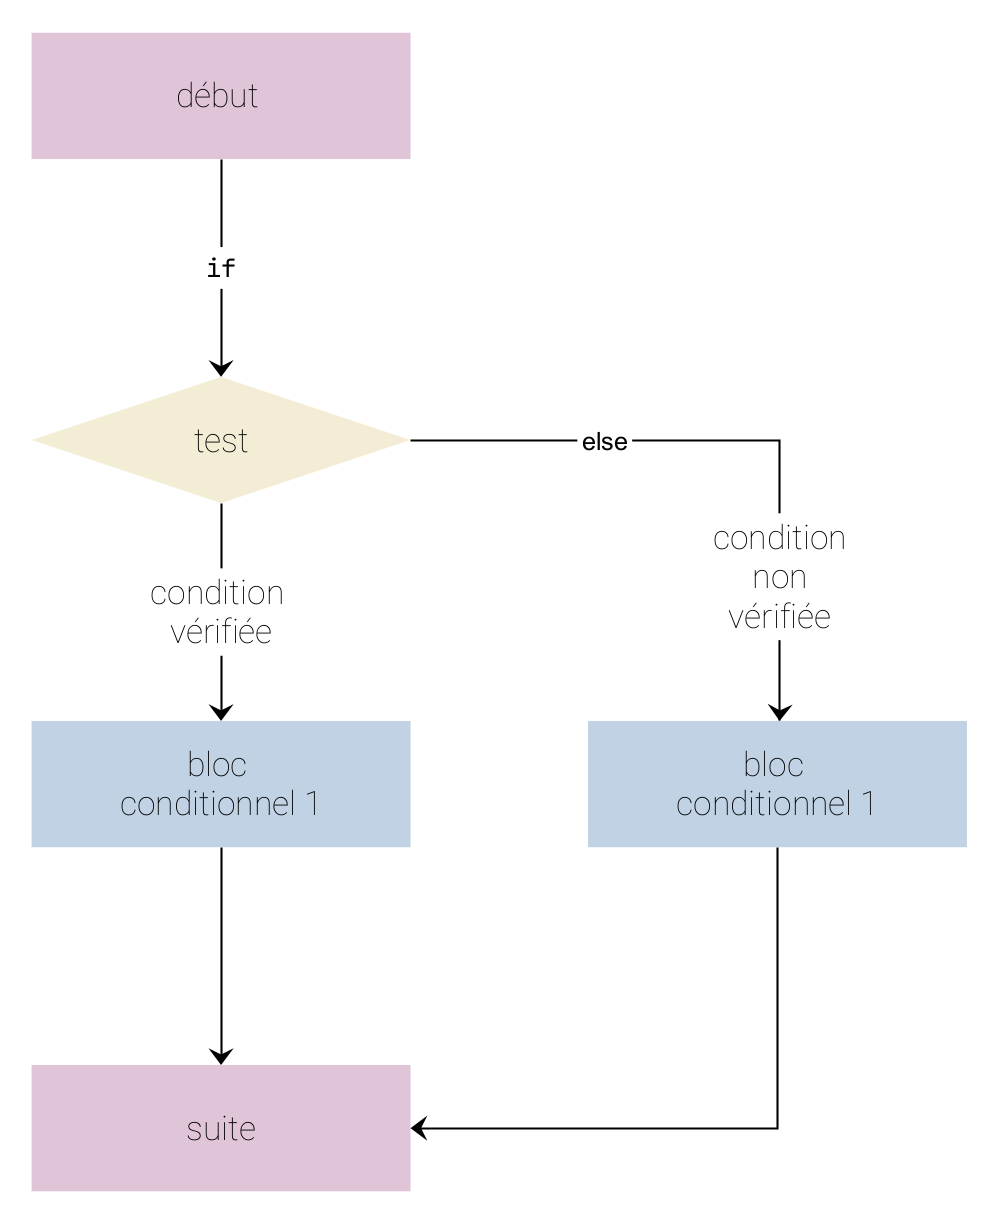
\includegraphics[height=10cm]{img/ifelse}
\end{center}

\begin{pyc}
	\begin{minted}{python}
print('Bonjour')
age = int(input('Entrez votre age : '))
if age >= 18:
    print('Vous etes majeur')
else:
    print('Vous etes mineur.')
print('Au revoir.')
\end{minted}
\end{pyc}

Voici un exemple de fonctionnement d'un test \pythoninline{if...elif...} :
\begin{pyc}
	\begin{minted}{python}
print('Bonjour')
prenom = input('Entrez un prénom : ')
if prenom == 'Robert':
    print("Robert, c'est le prénom de mon grand-père.")
elif prenom == 'Raoul':
    print("Mon oncle s'appelle Raoul.")
elif prenom == 'Médor':
    print("Médor, comme mon chien !")
else:
    print("Connais pas")
print('Au revoir.')
\end{minted}
\end{pyc}
Et voici un schéma décrivant son fonctionnement :
\begin{center}
	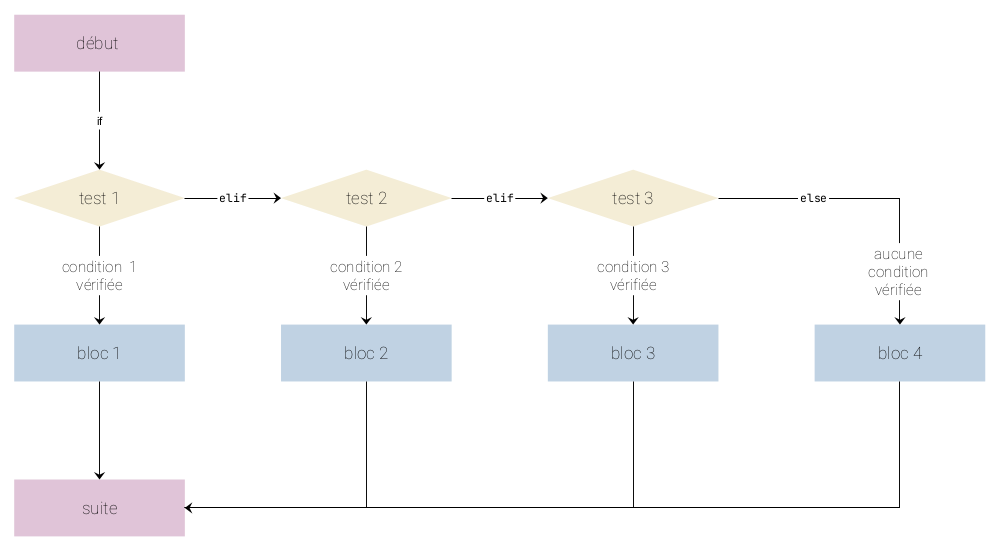
\includegraphics[width=\linewidth]{img/ifelifelse}
\end{center}



On peut bien sûr inclure autant de \pythoninline{elif} que nécessaire.

\section{Exercices}

%----------------------------------------------------------------------
\begin{exercice}
	\'Ecrire un script qui demande son âge à l'utilisateur puis qui affiche \pythoninline{'Bravo pour votre longévité.'} si celui-ci est supérieur à 90.
\end{exercice}

\begin{exercice}[]
	\'Ecrire un script qui demande un nombre à l'utilisateur puis affiche si ce nombre est pair ou impair.
\end{exercice}
%----------------------------------------------------------------------
\begin{exercice}
	\'Ecrire un script qui demande l'âge d'un enfant à l'utilisateur puis qui l'informe ensuite de sa catégorie :
	\begin{itemize}
		\item   trop petit avant 6 ans;
		\item   poussin de 6 à 7 ans inclus;
		\item   pupille de 8 à 9 ans inclus;
		\item   minime de 10 à 11 ans inclus;
		\item   cadet à 12 ans et plus;
	\end{itemize}
\end{exercice}
%----------------------------------------------------------------------

\begin{exercice}
	\'Ecrire un script qui demande une note sur 20 à l'utilisateur puis vérifie qu'elle est bien comprise entre 0 et 20. Si c'est le cas rien ne se produit mais sinon le programme devra afficher un message tel que \pythoninline{'Note non valide.'}.
\end{exercice}

\begin{exercice}
	\'Ecrire un script qui demande un nombre à l'utilisateur puis affiche s'il est divisible par 5, par 7 par aucun ou par les deux de ces deux nombres.
\end{exercice}
%----------------------------------------------------------------------
\begin{exercice}
	En reprenant l'exercice du chapitre 1 sur les numéros de sécurité sociale, écrire un script qui demande à un utilisateur son numéro de sécurité sociale, puis qui vérifie si la clé est valide ou non.
\end{exercice}


%----------------------------------------------------------------------
\begin{exercice}
	\'Ecrire un script qui résout dans $\R$ l'équation du second degré $ax^2+bx+c=0$.\\
	On commencera par \pythoninline{from math import sqrt} pour utiliser la fonction \pythoninline{sqrt}, qui calcule la racine carrée d'un \pythoninline{float}.

	On rappelle que lorsqu'on considère une équation du type $ax^2+bx+c=0$
	\begin{itemize}
		\item   si $a=0$ ce n'est pas une équation de seconde degré;
		\item   sinon on calcule $\Delta = b^2-4ac$ et
		      \begin{itemize}
			      \item   Si $\Delta<0$ l'équation n'a pas de solutions dans $\R$;
			      \item   Si $\Delta=0$ l'équation admet pour unique solution $\dfrac{-b}{2a}$;
			      \item   Si $\Delta>0$ l'équation admet 2 solutions : $\dfrac{-b-\sqrt{\Delta}}{2a}$ et $\dfrac{-b+\sqrt{\Delta}}{2a}$.
		      \end{itemize}
	\end{itemize}
	Pour vérifier que le script fonctionne bien on pourra tester les équations suivantes :
	\begin{itemize}
		\item   $2x^2+x+7=0$ (pas de solution dans $\R$);
		\item   $9x^2-6x+1=0$ (une seule solution qui est $\dfrac{1}{3}$);
		\item   $x^2-3x+2$ (deux solutions qui sont 1 et 2).
	\end{itemize}
\end{exercice}

%----------------------------------------------------------------------
\begin{exercice}
	L'opérateur \pythoninline{nand} est défini de la manière suivante : si \pythoninline{A} et \pythoninline{B} sont deux booléens alors
	\begin{center}
		\pythoninline{A nand B} vaut \pythoninline{not (A and B)}
	\end{center}
	Construire la table de vérité de \pythoninline{nand} en complétant :
	\begin{center}

		\begin{tabular}{|c|c|c|c|}
			\hline
			\rowcolor{UGLiOrange}{\boxfont\color{white} A} & {\boxfont\color{white} B} & {\boxfont\color{white} A and B} & {\boxfont\color{white} not (A and B)} \\
			\hline
			\pythoninline{False}                           & \pythoninline{False}      &                                 &                                       \\
			\hline
			\pythoninline{False}                           & \pythoninline{True}       &                                 &                                       \\
			\hline
			\pythoninline{True}                            & \pythoninline{False}      &                                 &                                       \\
			\hline
			\pythoninline{True}                            & \pythoninline{True}       &                                 &                                       \\
			\hline
		\end{tabular}
	\end{center}
\end{exercice}


